%!TEX root=ast2016.tex

\begin{figure}[t]
  \centering

  \begin{tabular}{c c}

    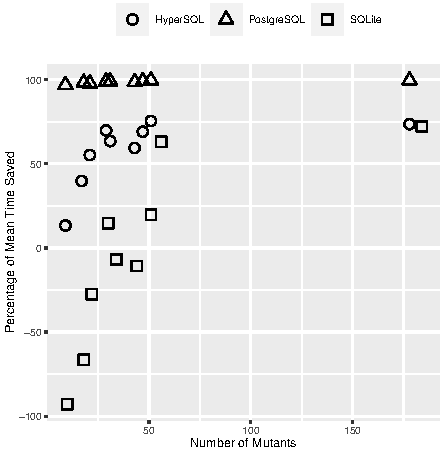
\includegraphics[scale=1.0]{graphics/graphic_scatterplot_nummutants_percentage.pdf} &
    % 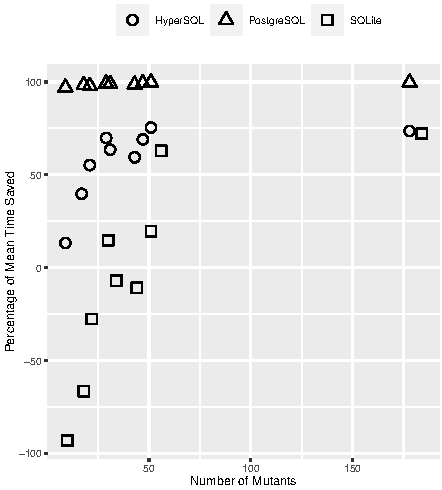
\includegraphics[scale=1.0]{graphics/graphic_scatterplot_numtests_percentage.pdf}

  \end{tabular}

  \caption{Scatter plot of the percentage of mean time saved for the number of mutants (left) and tests (right).}
  \label{fig:graphic_scatterplot_mutantstests_percentagetimesaved}

  {\small \justifying{ \noindent In these scatter plots, a specific point corresponds to the percentage of mean time
      saved for a given number of mutants (left plot) or tests (right plot), across all three of the database management
      systems. For a detailed description of how to calculate the values on the vertical axis, please refer to
      Section~\ref{sec:experimental-setup}.  } \par}

  \vspace*{-1em}

\end{figure}
